\documentclass[main.tex]{subfiles}
\begin{document}
\section{Appliquer une procédure}
%%%%%%%%%%%%%%%%%%%%%%%%%%%%%%%%%%%%%%%
% EXERCICE
\begin{exercise}[points=5]
    Le diagramme à barre ci-dessous donne la répartition des notes obtenues à un contrôle de mathématiques sur 20 points par les élèves de 4 TQ.
    \begin{center}
        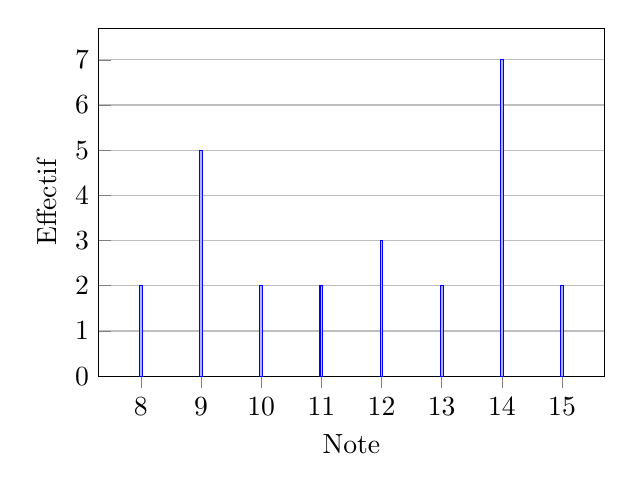
\begin{tikzpicture}
            \begin{axis} [
                ybar,
                height=6cm,
                width=8cm,
                xlabel={Note},
                ylabel={Effectif},
                ymin=0,
                xtick distance = 1,
                ytick distance = 1,
                %xtick={8,...,15},
                %ytick={1,...,7},
                ymajorgrids,
                xtick pos=bottom,
                ytick pos=left,
                bar width=1pt]
                \addplot coordinates {
                    (8,2)
                    (9,5)
                    (10,2)
                    (11,2)
                    (12,3)
                    (13,2)
                    (14,7)
                    (15,2)
                };
                \end{axis}
        \end{tikzpicture}
    \end{center}
    \begin{enumerate}
        \item Combien d'élèves y-a-t-il dans cette classe ?
        \item Quelle est la note la plus observée à ce contrôle ? En termes statistiques, comment appelle-t-on cette valeur ?
        \item Quelle est la note moyenne de la classe à ce contrôle ?
        \item Quelle est la note médiane de la classe à ce contrôle ?
        \item Si l'on considère que les élèves ont réussi s'ils ont obtenu la moitié ou plus, détermine le pourcentage de réussite de la classe.
    \end{enumerate}
\end{exercise}
% SOLUTION 
\begin{solution}
    \begin{enumerate}
        \item $2+5+2+2+3+2+7+2 = 25$. Il y a 25 élèves.
        \item $14$.
        \item $\dfrac{8\cdot 2+9\cdot 5+10\cdot 2+11\cdot 2+12\cdot 3+13\cdot 2+14\cdot 7+15\cdot 2}{22} = \dfrac{293}{22}=11,72$
        \item $12$
    \end{enumerate}
\end{solution}
%%%%%%%%%%%%%%%%%%%%%%%%%%%%%%%%%%%%%%%
% EXERCICE
\begin{exercise}[points=4]
    Dans une entreprise de \num{21} employés, le comptable a répertorié le montant des différents salaires dans le tableau ci-dessous.
    \begin{center}
        \begin{tblr}{hlines, vlines, columns={r, 1cm}, column{1}={l, 2cm}}
            Salaire (€) & \num{950} & \num{1250} & \num{1500} & \num{2500} & \num{3500} \\
            Effectif    & \num{4}   & \num{8}    & \num{6}    & \num{2}    & \num{1}
        \end{tblr}
    \end{center}
    \begin{enumerate}
        \item Calcule le salaire médian de cette entreprise.
        \item Calcule le salaire moyen de cette entreprise. Arrondis à l'unité.
        \item Quel est le salaire perçu par la majorité des employés ?
        \item Quel pourcentage des employés touche moins de \num{1500}~€ ? Arrondis à l'unité.
    \end{enumerate}
\end{exercise}
% SOLUTION
\begin{solution}
    \begin{enumerate}
        \item 
        La médiane est la 11\ieme valeur : \SI{1250}{\EUR}. La moitié des employés gagne \SI{1250}{\EUR} ou moins et l'autre moitié gagne \SI{1250}{\EUR} ou plus.
        \item 
        $\dfrac{\num{950}\cdot 4 + \num{1250} \cdot 8 + \num{1500} \cdot 6 + \num{2500} \cdot 2 + \num{3500} \cdot 1}{21} = \dfrac{\num{31300}}{21}\approx\SI{1490}{\EUR}$. Si on redistribuait les salaires équitablement entre chaque employé, chacun gagnerait \SI{1490}{\EUR}.
        \item 
        La majorité des employés perçoit un salaire de \SI{1250}{\EUR}
        \item 
        $\dfrac{12}{21}\cdot 100 = 57\%$.
    \end{enumerate}
\end{solution}

%%%%%%%%%%%%%%%%%%%%%%%%%%%%%%%%%%%%%%%
% EXERCICE
\begin{exercise}[points=2]
    Détermine la valeur de $a$ pour que la moyenne de cette série statistique soit égale à 15. Note ta démarche.
    \[17,\ 12,\ a,\ 10\]
\end{exercise}
% SOLUTION
\begin{solution}

\end{solution}
%%%%%%%%%%%%%%%%%%%%%%%%%%%%%%%%%%%%%%%
% EXERCICE
\begin{exercise}[points=4]
    Voici les résultats obtenus lors de plusieurs lancés de dé.
    \begin{center}
        \numlist{6;1;5;3;2;1;6;4;1;3;4;5;4;3;5;3;5;1;2;6}
    \end{center}
    \begin{enumerate}
        \item Réalisez un tableau dont voici les en-têtes. Arrondissez au centième.
              \begin{center}
                  \begin{tblr}{hlines, vlines, rows={m}}
                      Modalités & Effectifs & Effectis cumulés & Fréquences & Fréquences  cumulées \\
                  \end{tblr}
              \end{center}

        \item Représente par un graphique cette série. N'oubliez pas de nommer vos axes et votre graphique.
        \item Pour cette série détermine la moyenne et la médiane.
    \end{enumerate}
\end{exercise}
% SOLUTION
\begin{solution}

\end{solution}
\end{document}